%**********************************************************
The remote system is responsible for the communication between the local systems and the internet. In this project, the internet is used to maintain a cloud database, so the remote system does the data bridge between the network of street lampposts and a cloud. As one can see in figure \ref{fig:rs_overview}, the remote system is composed by the main process and a daemon process \textit{dServerSend}. The main process may be composed of a server and varoius clients, being the messages from each client received and processed in this process. The messages are sent to the clients in the daemon process \textit{dServerSend}. The communication between the two processes is done using message queues, so when a command is received and successfully parsed, the main process sends the command output to the daemon using the message queue.

\begin{figure}[H]
	\centering
%	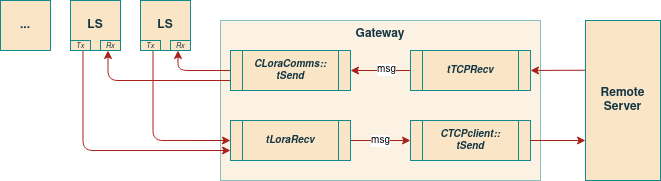
\includegraphics[width=.3\textwidth]{09sw_specification/RS/overview}
	\caption{Inter-process Communication between Main Process and Daemon.}
	\label{fig:rs_overview}
\end{figure}

%**********************************************************
\subsection{Class Diagram}
In figure \ref{fig:rs_classDiag} is represented the class diagram of the remote system. The class \textit{CTCPServer} is the main class of the system, that initializes the objects of each class. 

\begin{itemize}
	\item \textbf{CTCPServer:} main class, responsible for creating the server, the client objects, each time a client connects to the server and for sending the messages to the clients;
	\item \textbf{CClient:} client class, stores the clients information and receives their messages;
	\item \textbf{CDataBase:} provides an interface between the server and the database.

\end{itemize}

\begin{figure}[H]
	\centering
%	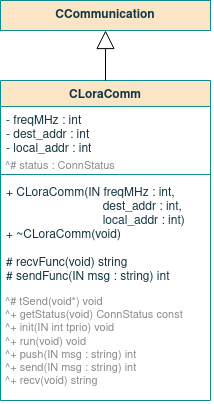
\includegraphics[width=.6\textwidth]{09sw_specification/RS/class}
	\caption{Inter-process Communication between Main Process and Daemon.}
	\label{fig:rs_classDiag}
\end{figure}

%****************************
\myparagraph{Class CTCPServer}
This class is responsible for creating the server, using \textit{createServer} function, allowing multiple clients to connect and send them messages, with the thread \textit{tSend}. When a client connects to the server, this class creates a new instance of the class \textit{CClient}. Each client can be of a different type of device like website, mobile application or gateway. The clients are assigned to their respective list of clients that are \textit{webSList}, \textit{appList} and \textit{gatewayList}, respectively. To do the interface with the database, this class also has an instance of the class database. In figure \ref{fig:CTCPServer}, one can see the class \textit{CTCPServer} diagram.

\begin{figure}[H]
	\centering
	%	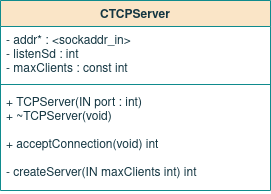
\includegraphics[width=.6\textwidth]{09sw_specification/RS/CTCPServer}
	\caption{Class Diagram: CTCPServer.}
	\label{fig:CTCPServer}
\end{figure}

\myparagraph{Class CClient}
The class \textit{CClient}, represented in figure \ref{}

\begin{figure}[H]
	\centering
	%	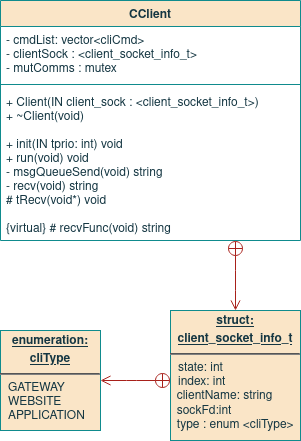
\includegraphics[width=.6\textwidth]{09sw_specification/RS/CClient}
	\caption{Class Diagram: CClient.}
	\label{fig:CTCPServer}
\end{figure}

%**********************************************************
\subsection{Task Overview}
One can define and describe briefly how the remote system is implemented, making use of threads and processes. 

\begin{itemize}
	\item \textbf{t}
\end{itemize}

%**********************************************************
\subsection{Task Priority}

%**********************************************************
\subsection{Task Synchronization}

\myparagraph{Condition Variables}
The condition variables used in this system are listed below.

\begin{itemize}
	\item
		
\end{itemize}

\myparagraph{Mutexes}
The mutexes used in this system are listed bellow.

\begin{itemize}
	\item 
	
\end{itemize}

\myparagraph{Semaphores}

\subsection{Task Communication}
\myparagraph{Message Queues}
\myparagraph{Signals}

%**********************************************************
\subsection{Flowcharts}


%**********************************************************
\subsection{Start-up Process}

%**********************************************************
\subsection{Shutdown Process}
